% =====================================================================
% AAAI 2027 submission build of:
%   "DHRP: A Differentiable Hierarchical Risk Parity Architecture
%    and Multi-Universe Portfolio Benchmark"
%
% Track:  Main Technical Track
% Format: two-column, 10pt Times, US Letter
% Pages:  7 body + unlimited references
%
% Style files (place in this directory):
%   aaai2026.sty  -- proxy until AAAI 2027 author kit is released.
%                    When released, download from https://aaai.org/authorkit27/
%                    and replace aaai2026.sty with aaai2027.sty, then update
%                    \usepackage below accordingly.
%   aaai2026.bst  -- same: replace with aaai2027.bst when released.
%   NOTE: Do NOT modify aaai2026.sty -- AAAI prohibits any modification.
%
% Build:
%   pdflatex main_aaai_submission ; bibtex main_aaai_submission ; \
%     pdflatex main_aaai_submission ; pdflatex main_aaai_submission
%
% Submission options:
%   [submission]   : anonymous (hides author block) -- USE THIS FOR SUBMISSION
%   (no option)    : camera-ready (shows author block)
% =====================================================================
\documentclass[letterpaper]{article}

% For double-blind submission upload, re-add the [submission] option:
%   \usepackage[submission]{aaai2026}
\usepackage{aaai2026}   % swap to aaai2027 when kit releases
\usepackage{times}
\usepackage{helvet}
\usepackage{courier}
\usepackage[hyphens]{url}
\usepackage{graphicx}
\usepackage{amsmath, amssymb, amsthm}
\usepackage{booktabs}
\usepackage{natbib}
\usepackage{algorithm}
\usepackage{algorithmic}
\usepackage{multirow}
\usepackage{xcolor}
\usepackage{microtype}
\usepackage{tikz}
\usetikzlibrary{positioning, arrows.meta, shapes.geometric, calc}

\frenchspacing
\setlength{\pdfpagewidth}{8.5in}
\setlength{\pdfpageheight}{11in}

\newtheorem{proposition}{Proposition}

\graphicspath{{figures/}{../results/figures/}}

\title{DHRP: A Differentiable Hierarchical Risk Parity Architecture and Multi-Universe Portfolio Benchmark}

% In [submission] mode, the author block is suppressed automatically.
\author{Jose Luis Amador Jaime\\
Independent Researcher}

\begin{document}
\maketitle

\begin{abstract}
Hierarchical Risk Parity (HRP) builds portfolios through agglomerative
clustering and recursive bisection, two discrete operations that block
gradient flow and keep HRP outside end-to-end learning pipelines. We
introduce DHRP, a differentiable relaxation that replaces hard clustering
with a temperature-scaled soft-gating binary tree, a learned
asset-to-leaf assignment, and an inverse-volatility blend, trained
jointly against a multi-objective utility with an HRP-anchored
regularizer. We evaluate on DHRP-8, a new benchmark covering eight ETF
universes, eight headline allocators, and ten seeds, with Probabilistic
Sharpe Ratios, factor alphas, SPA and MCS tests, transaction-cost curves,
and Croissant metadata. DHRP achieves the best out-of-sample Sharpe in
commodities (1.304, PSR 0.999) and crypto (1.290, PSR 0.991) and beats
classical HRP in six of eight universes. A FinBERT text extension,
LLM-DHRP, gives no statistical benefit and regresses in two of three
text-covered universes; we report this negative result in full.
\end{abstract}


\section{Introduction}
\label{sec:intro}

Mean-variance optimization \citep{Markowitz1952} remains the canonical
formulation of portfolio choice, but its weights are sensitive to
estimation error, to the point that the naive 1/N rule is hard to beat
out of sample \citep{DeMiguel2009}. Hierarchical Risk Parity
\citep{LopezdePrado2016} sidesteps covariance inversion entirely: it
clusters assets by correlation distance and then splits risk down the
resulting dendrogram by recursive bisection. The recipe is simple,
stable under noisy covariance estimates \citep{Raffinot2018}, and widely
deployed. It is also frozen. Both the clustering and the bisection are
discrete, so no gradient can pass through them, and HRP cannot be trained
jointly with upstream feature extractors or tuned against a downstream
objective.

A growing body of work makes optimization layers differentiable, from
quadratic programs \citep{Amos2017} to general convex programs
\citep{Agrawal2019} and end-to-end mean-variance solvers
\citep{Pan2024BPQP}, yet hierarchical allocators have been left out of
this development. We close the gap with DHRP, which replaces HRP's two
discrete stages with a temperature-scaled soft-gating binary tree and a
learned soft assignment of assets to leaves, blended with
inverse-volatility weights and trained end to end. An HRP regularizer
warm-starts the model from classical HRP weights and anneals over
training; ablations show it is load-bearing. We frame DHRP as an
HRP-inspired relaxation rather than an exact differentiable clone, and we
state precisely where the correspondence breaks.

Evaluation practice in deep portfolio research is a second gap. Many
papers report a single seed on a single universe, even though seed
variance in neural allocators can exceed the gaps between methods, a
problem documented for ML benchmarks more broadly
\citep{Reuel2024BetterBench}. We therefore release DHRP-8: eight ETF
universes, eight headline allocators plus four supplementary deep
baselines, ten seeds per neural method, and a five-family statistical
battery built around the Probabilistic Sharpe Ratio \citep{Bailey2012PSR},
factor alphas, and the SPA and MCS multi-method tests
\citep{Hansen2005,HansenLundeNason2011}.

Finally, we test the obvious next step honestly. LLM-DHRP fuses a FinBERT
summary of asset-attributed news \citep{Huang2023} into the tree through
a gated residual. Under ten-seed reporting it delivers no statistical
benefit and regresses in two of the three universes with text coverage.
Rather than tuning until the number turns positive, we report the failure
and diagnose its mechanisms, joining recent benchmarks that find LLM
components add little to quantitative trading and forecasting
\citep{Tan2024AreLMs,Chen2025StockBench,Xie2024FinBen}.

\paragraph{Contributions.}
\begin{itemize}\itemsep0.05em
\item \textbf{DHRP}, a fully differentiable HRP-inspired allocator built
  from a soft-gating binary tree, a learned asset-to-leaf assignment, and
  an inverse-volatility blend, anchored by an annealed HRP regularizer.
  It beats classical HRP in six of eight universes and attains the best
  Sharpe in commodities ($1.304 \pm 0.095$, PSR 0.999) and crypto
  ($1.290 \pm 0.052$, PSR 0.991).
\item \textbf{DHRP-8}, a multi-universe benchmark with ten-seed error
  bars, PSR, Fama-French alphas, SPA and MCS tests, transaction-cost
  sensitivity, and Croissant 1.1 metadata, released with frozen
  dependencies and a single-command reproduction script.
\item \textbf{An honest negative ablation.} LLM-DHRP, a FinBERT-augmented
  variant, shows no statistically reliable gain, and we trace the failure
  to news coverage sparsity, embedding anisotropy that survives temporal
  aggregation, and warm-start instability.
\end{itemize}


\section{Related Work}
\label{sec:related}

\paragraph{HRP and differentiable optimization.}
HRP \citep{LopezdePrado2016} and its linkage variants \citep{Raffinot2018}
belong to the risk-budgeting family alongside equal risk contribution
\citep{Maillard2010,Roncalli2013} and maximum diversification
\citep{Choueifaty2008}; all aim to avoid the estimation fragility of
mean-variance weights \citep{Markowitz1952,Ledoit2004,DeMiguel2009}.
Differentiable optimization layers \citep{Amos2017,Agrawal2019,Bolte2021}
have reached portfolio construction through end-to-end mean-variance
backpropagation \citep{Pan2024BPQP} and m-sparse Sharpe maximization
\citep{Lin2024MSparse}, but hierarchical allocation has remained outside
this toolkit. Closest to us is concurrent work embedding HRP in a
reinforcement-learning loop with Bayesian sector shrinkage
\citep{KangTian2025RLBHRP}. That approach keeps the HRP computation hard
and learns around it with RL, and it is evaluated on US equities only;
DHRP instead makes the hierarchy itself differentiable, trains by plain
gradient descent, and is benchmarked across eight asset classes.

\paragraph{Soft trees and decision-focused learning.}
Our gating tree descends from soft decision trees \citep{FrosstHinton2017},
oblivious neural ensembles \citep{Popov2020NODE}, differentiable tree
ensembles \citep{Hazimeh2020TreeEnsemble}, and sparsely gated mixtures of
experts \citep{Shazeer2017}; differentiable tree structures remain an
active topic \citep{Mao2025DiffTree}. Training allocation weights against
a downstream financial objective places DHRP within decision-focused
learning \citep{Wilder2019,Elmachtoub2022SPO,Donti2017}, where recent
portfolio instances include deep declarative risk budgeting
\citep{ParraDiaz2025} and decision-focused minimum variance
\citep{KimLee2025DFL}.

\paragraph{LLMs in finance and benchmark precedents.}
Domain language models such as FinBERT \citep{Araci2019,Huang2023} and
BloombergGPT \citep{Wu2023BloombergGPT} have fueled text-augmented trading
systems, though reported gains are often single-seed \citep{Kirtac2025}
and deserve caution. A recent wave of benchmarks reaches sobering
conclusions: most LLM trading agents fail to beat buy-and-hold
\citep{Chen2025StockBench}, LLMs are weak financial forecasters
\citep{Xie2024FinBen}, removing the LLM component can improve time-series
models outright \citep{Tan2024AreLMs}, and live prediction-market
evaluation is similarly mixed \citep{Cheng2026PolyBench}. Our negative
ablation adds a multi-seed portfolio-allocation data point to this
literature.

\paragraph{Multi-seed and PSR reporting.}
Sample Sharpe ratios overstate skill under non-normal returns and short
samples; the Probabilistic Sharpe Ratio \citep{Bailey2012PSR} and the
deflated Sharpe ratio \citep{Bailey2014DSR} correct for this. Benchmark
audits also find that error bars and reproducibility metadata are
routinely missing \citep{Reuel2024BetterBench}. DHRP-8 therefore reports
ten-seed means with standard deviations, HAC t-statistics
\citep{NeweyWest1987}, factor alphas \citep{FamaFrench2015,Carhart1997},
stationary-bootstrap Sharpe-difference tests \citep{PolitisRomano1994}
with Holm correction \citep{Holm1979} and Diebold-Mariano statistics
\citep{DieboldMariano1995}, the SPA test \citep{Hansen2005}, model
confidence sets \citep{HansenLundeNason2011}, and Croissant 1.1 metadata
\citep{Akhtar2024Croissant}.


\section{Method}
\label{sec:method}

DHRP maps a price feature vector $x_t$ and an annualized covariance matrix
$\Sigma_t$ to portfolio weights through four stages: feature fusion, a
soft-gating tree, a soft asset assignment, and an inverse-volatility
blend. Figure~\ref{fig:arch} gives an overview; we describe each stage in
turn.

% TikZ architecture diagram for DHRP + LLM-DHRP (inlined into main.tex).
\begin{figure*}[t]
\centering
\resizebox{\textwidth}{!}{%
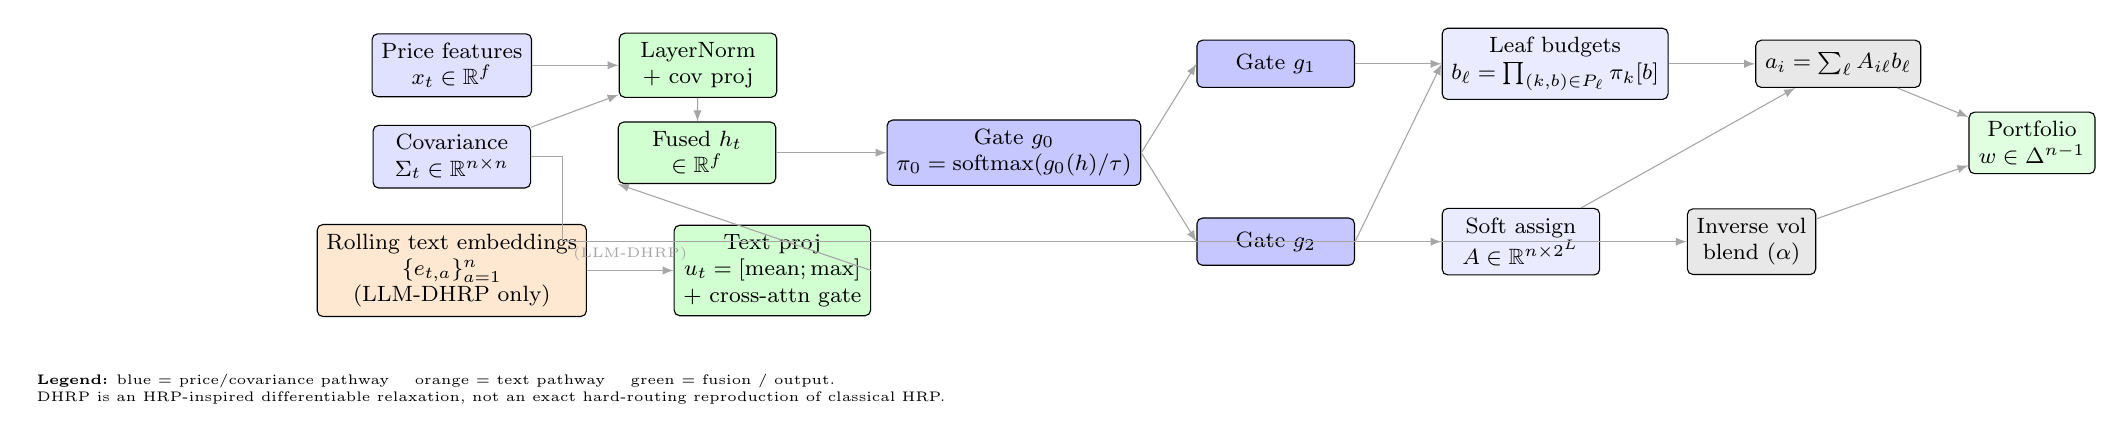
\begin{tikzpicture}[
    node distance=0.9cm,
    every node/.style={font=\small},
    box/.style={draw, rounded corners=2pt, minimum width=2.0cm, minimum height=0.6cm,
                align=center, font=\footnotesize},
    txt/.style={box, fill=orange!18},
    price/.style={box, fill=blue!12},
    cov/.style={box, fill=blue!12},
    fuse/.style={box, fill=green!18},
    tree/.style={box, fill=blue!22},
    outbox/.style={box, fill=gray!18, minimum width=1.6cm},
    arrow/.style={->, >=latex, thin, gray!70},
    dashedarrow/.style={->, >=latex, thin, gray!50, dashed},
]

% --- Inputs (left column) ---
\node[price]                              (x)   {Price features\\ $x_t \in \mathbb{R}^{f}$};
\node[cov,    below=0.35cm of x]          (S)   {Covariance\\ $\Sigma_t \in \mathbb{R}^{n\times n}$};
\node[txt,    below=0.45cm of S]          (T)   {Rolling text embeddings\\ $\{e_{t,a}\}_{a=1}^n$\\ (LLM-DHRP only)};

% --- Feature fusion (middle column) ---
\node[fuse,   right=1.1cm of x]           (norm) {LayerNorm\\ + cov proj};
\node[fuse,   right=1.1cm of T]           (txp)  {Text proj\\ $u_t=[\mathrm{mean};\mathrm{max}]$\\ + cross-attn gate};
\node[fuse,   right=1.1cm of S, yshift=0.05cm] (h) {Fused $h_t$\\ $\in \mathbb{R}^{f}$};

% --- Soft-gating tree (right column) ---
\node[tree,   right=1.4cm of h]           (g0)  {Gate $g_0$\\ $\pi_0 = \mathrm{softmax}(g_0(h)/\tau)$};
\node[tree,   below right=0.4cm and 0.7cm of g0] (g2) {Gate $g_2$};
\node[tree,   above right=0.4cm and 0.7cm of g0] (g1) {Gate $g_1$};

% --- Leaf budgets + assignment + output ---
\node[box,    fill=blue!8, right=1.1cm of g1] (leaves) {Leaf budgets\\ $b_\ell = \prod_{(k,b)\in P_\ell} \pi_k[b]$};
\node[box,    fill=blue!8, right=1.1cm of g2] (assign) {Soft assign\\ $A \in \mathbb{R}^{n\times 2^L}$};
\node[outbox,    right=1.1cm of leaves]      (alloc) {$a_i = \sum_\ell A_{i\ell} b_\ell$};
\node[outbox,    right=1.1cm of assign]      (vol)   {Inverse vol\\ blend ($\alpha$)};
\node[outbox,    fill=green!12, below right=0.3cm and 0.6cm of alloc] (w) {Portfolio\\ $w \in \Delta^{n-1}$};

% --- Arrows ---
\draw[arrow] (x) -- (norm);
\draw[arrow] (S) -- (norm);
\draw[arrow] (T) -- (txp) node[midway, above, font=\tiny]{(LLM-DHRP)};
\draw[arrow] (norm) -- (h);
\draw[arrow] (txp.east) -- (h.south west);
\draw[arrow] (h) -- (g0);
\draw[arrow] (g0.east) -- (g1.west);
\draw[arrow] (g0.east) -- (g2.west);
\draw[arrow] (g1.east) -- (leaves.west);
\draw[arrow] (g2.east) -- (leaves.west);
\draw[arrow] (g2.east) -- (assign.west);
\draw[arrow] (leaves) -- (alloc);
\draw[arrow] (assign) -- (alloc);
\draw[arrow] (S.east) -- ++(0.4,0) |- (vol.west);
\draw[arrow] (alloc) -- (w);
\draw[arrow] (vol)   -- (w);

% --- Legend (compact) ---
\node[below=0.6cm of T, xshift=0.5cm, font=\tiny, align=left] {%
  \textbf{Legend:} blue = price/covariance pathway \quad orange = text pathway \quad green = fusion / output.\\
  DHRP is an HRP-inspired differentiable relaxation, not an exact hard-routing reproduction of classical HRP.};
\end{tikzpicture}%
}
\caption{DHRP and LLM-DHRP architecture. Price features, covariance,
and (optional) global text summaries are fused via LayerNorm and a
gated cross-attention residual into $h_t$, which routes through a
temperature-scaled binary gating tree. Leaf budgets are combined with a
learned soft assignment matrix and blended with inverse-volatility
weights to produce portfolio weights $w \in \Delta^{n-1}$.}
\label{fig:arch}
\end{figure*}


\subsection{DHRP: differentiable soft-gating tree}
\label{sec:dhrp_layer}

Covariance information enters through a dedicated projection. A small MLP
encodes the normalized, flattened covariance $\Sigma_t$, and the result is
fused with the price features $x_t$ under LayerNorm to produce a hidden
vector $h_t$. Conditioning on the full covariance, rather than on
volatilities alone, lets the downstream gates react to changes in
correlation structure, which is the quantity classical HRP clusters on.
\begin{equation}
h_t = \mathrm{LayerNorm}\left(x_t + f_{\text{cov}}\!\left(
\mathrm{vec}(\Sigma_t)/(\|\Sigma_t\|_\infty + \epsilon)\right)\right).
\end{equation}

The hidden vector drives a perfect binary tree of depth $L$, with $2^L$
leaves and $2^L - 1$ internal nodes. Each internal node $k$ applies a gate
to $h_t$ and emits a two-way temperature-scaled softmax $\pi_k$, where the
per-node temperature $\tau_k = \exp(\theta_k)$ is clamped to $(0.1, 5.0]$.
\begin{equation}
\pi_k = \mathrm{softmax}(g_k(h_t) / \tau_k),
\quad \tau_k = \exp(\theta_{\tau,k}) \in (0.1, 5.0].
\label{eq:gates}
\end{equation}
A leaf's budget is the product of gate probabilities along its
root-to-leaf path $P_\ell$, namely
$p_\ell = \prod_{(k, b) \in P_\ell} \pi_k[b]$, renormalized by a learned
leaf prior $\beta = \mathrm{softmax}(\theta_\beta)$ to give
$b_\ell = \beta_\ell p_\ell / \sum_j \beta_j p_j$. Low temperatures
sharpen the gates toward hard routing while high temperatures spread risk
across subtrees, and the temperatures are themselves learned, so the
network chooses how decisive each split should be.

Leaves are not tied to fixed clusters. A learnable matrix
$A \in \mathbb{R}^{n \times 2^L}$ with row-wise softmax distributes leaf
budgets to assets, yielding soft allocations
$a_i = \sum_\ell \mathrm{softmax}(A_{i,:})_\ell\, b_\ell$; the assignment
trains jointly with the gates, so the tree discovers its own grouping
rather than inheriting one from a linkage rule. The final weight blends
$a_i$ with an inverse-volatility weight through a learned coefficient
$\alpha = \sigma(\theta_\alpha)$, after which weights are clipped to be
nonnegative and renormalized. The blend keeps the allocator near a
sensible risk-parity baseline early in training while leaving the learned
path free to dominate where it helps.
\begin{equation}
w_i = \alpha \cdot a_i + (1-\alpha) \cdot \frac{1/\sigma_i}{\sum_j 1/\sigma_j},
\qquad \alpha = \sigma(\theta_\alpha),
\label{eq:blend}
\end{equation}

Training minimizes a multi-objective loss: the negative of a CRRA utility,
a smooth Sharpe term, and an entropy bonus, augmented by four penalties.
An HRP regularizer $\lVert w - w_{\mathrm{HRP}} \rVert^2$ warm-starts the
model from classical HRP weights, with its coefficient $\lambda_h$
following a curriculum from 0.3 down to 0.05 so the anchor relaxes as
training proceeds. A risk penalty $w^\top \Sigma w$, an HHI concentration
penalty, and a turnover penalty complete the objective. The HRP term is
load-bearing rather than decorative: removing it drops commodity Sharpe by
$0.32 \pm 0.06$ across seeds, as the ablations below show.
\begin{align}
\mathcal{L} &= -(\mathrm{CRRA} + \mathrm{Sharpe} + \lambda_e \mathrm{Entropy}) \notag\\
&\quad + \lambda_h \|w - w_{\text{HRP}}\|_2^2 + \lambda_r w^\top \Sigma w \notag\\
&\quad + \lambda_c \mathrm{HHI}(w) + \lambda_t \mathrm{TO}(w).
\end{align}

\paragraph{Architecture scope.}
DHRP is an HRP-inspired relaxation, not an exact differentiable clone of
\citet{LopezdePrado2016}. The hard-routing limit of the gating tree does
not reproduce recursive HRP bisection across all subtrees, and at low
temperature the softmax gates collapse mass onto a single leaf rather than
recovering a balanced split. What the architecture preserves is the
inductive bias: hierarchical risk budgeting over a tree conditioned on
correlation structure, with the HRP regularizer supplying the explicit
anchor to the classical solution. Claims in this paper should be read
accordingly. A row-wise entropy-regularized reading of the assignment
matrix connects it to the Sinkhorn literature, though our implementation
enforces only row-stochasticity rather than the full bi-stochastic
iteration.

\subsection{LLM-DHRP: text-augmented allocation}
\label{sec:llm_dhrp_arch}

LLM-DHRP adds a text pathway. For each asset $a$ we collect headlines over
a 90-day rolling window, encode each with FinBERT \citep{Huang2023} into
768-dimensional embeddings, average within the window to obtain $e_{t,a}$,
and L2-normalize. The per-asset vectors are then pooled into a global
summary $u_t$ by concatenating the cross-asset mean and cross-asset max,
\begin{equation}
u_t =
\left[
\frac{1}{n}\sum_{a=1}^{n}\tilde e_{t,a};\;
\max_{a=1,\ldots,n}\tilde e_{t,a}
\right]\in\mathbb{R}^{2d_T},
\end{equation}
with $\tilde e_{t,a}=e_{t,a}/(\|e_{t,a}\|_2+\epsilon)$. A TextProjection
MLP maps $u_t$ into the price feature space, and a gated residual adds it
to $h_t$,
\begin{equation}
\hat h_t = h_t + g_{\text{text}} \cdot \mathrm{TextProj}(u_t),
\quad g_{\text{text}} = \sigma(\theta_g - 1.0),
\end{equation}
where the $-1.0$ bias suppresses text at initialization, and modality
dropout with $p = 0.1$ keeps the price path functional without it.
Training is two-phase: text and fusion parameters first with the price
path frozen, then all parameters at a reduced learning rate. The global
summary is a deliberate choice over per-asset cross-attention. News
coverage is sparse and skewed toward mega-caps, and pilot runs with
asset-token attention produced seed variance dominated by coverage gaps,
so we pool text into a single market-level signal instead.


\section{The DHRP-8 Benchmark}
\label{sec:benchmark}

\paragraph{Universes.}
Eight universes of 10 US-traded ETFs each: developed markets (DM),
emerging markets (EM), commodities, US sectors, global multi-asset, factor
ETFs, crypto, and bonds. All series have at least 12 years of daily
history, except crypto, which spans 2020 to 2026.

\paragraph{Methods.}
Eight headline allocators: six classical, deterministic methods (equal
weight, mean-variance, minimum variance, risk parity, maximum
diversification, and HRP) and two neural methods (DHRP and LLM-DHRP). Four
further deep allocators, an MLP with covariance projection, a Portfolio
Transformer \citep{KisielGorse2022}, PPO, and a decision-focused learner
\citep{KimLee2025DFL}, appear in the supplement, for 12 allocators in
total.

\paragraph{Multi-seed protocol.}
Training spans April 2012 to June 2020; the out-of-sample window runs from
July 2020 to April 2026, separated by a 5-day purge gap. Portfolios
rebalance every 5 days in commodities and crypto and every 21 days
elsewhere. Neural methods run with 10 seeds and are reported as mean $\pm$
standard deviation; classical methods are deterministic and contribute a
single value.

\paragraph{Statistical battery.}
Five families: PSR \citep{Bailey2012PSR}; HAC t-statistics
\citep{NeweyWest1987}; Fama-French three- and five-factor alphas plus
momentum \citep{FamaFrench2015,Carhart1997}; stationary block-bootstrap
pairwise Sharpe-difference tests \citep{PolitisRomano1994} with
Holm-Bonferroni correction \citep{Holm1979} and Diebold-Mariano tests
\citep{DieboldMariano1995}; and the SPA \citep{Hansen2005} and MCS
\citep{HansenLundeNason2011} multi-method tests at $\alpha = 0.05$.

\paragraph{Reproducibility.}
The release ships Croissant 1.1 metadata \citep{Akhtar2024Croissant},
frozen requirements, a single-command \texttt{reproduce\_all.sh}, and an
anonymous code URL.


\section{Results}
\label{sec:results}

\subsection{Multi-universe Sharpe summary}
\label{sec:results_main}

Table~\ref{tab:headline} summarizes out-of-sample Sharpe ratios. DHRP
performs best where correlation structure is rich and regimes shift:
commodities ($1.304 \pm 0.095$, PSR 0.999) and crypto
($1.290 \pm 0.052$, PSR 0.991), the top method in both universes. In
developed markets it reaches $0.446 \pm 0.056$ (PSR 0.856), the best of
the risk-parity family and ahead of mean-variance (0.333), equal weight
(0.255), and classical HRP (0.216). Classical methods keep the lead
elsewhere. Mean-variance dominates the global multi-asset universe (0.994,
PSR 0.990, against DHRP at $0.357 \pm 0.092$), EM (0.660 versus DHRP's
$0.469 \pm 0.004$), and sectors (0.861), while HRP is best in factors
(0.704, PSR 0.955). Overall DHRP beats classical HRP in six of eight
universes; the two losses, sectors ($0.677 \pm 0.050$ vs 0.698) and
factors ($0.682 \pm 0.033$ vs 0.704), both sit within 0.03 Sharpe. Bonds
are a failure case for every allocator: all methods lose money through the
2022-2023 rate-hike period, and DHRP's $-0.896 \pm 0.055$ (PSR 0.016)
still improves on HRP ($-1.176$) and equal weight ($-1.021$). The picture
supports an asset-class-contingent reading: no single method wins
everywhere, and the formal tests below agree.

% Auto-generated by scripts/generate_paper_tables.py - do not hand-edit
\begin{table*}[t]
\caption{Mean$\pm$std out-of-sample Sharpe across 10 seeds with Probabilistic Sharpe Ratio in brackets. Bold marks best method per universe; $\ast$ marks PSR $> 0.95$. Classical baselines are deterministic (no std).}
\label{tab:headline}
\centering
\setlength{\tabcolsep}{3pt}
\resizebox{\textwidth}{!}{%
\begin{tabular}{lcccccccc}
\toprule
Method & DM & EM & CMD & Sect & Glb & Fact & Cry & Bnd \\
\midrule
EW & 0.255 [0.730] & 0.479 [0.875] & 0.769 [0.967$^{\ast}$] & 0.706 [0.955$^{\ast}$] & 0.559 [0.911] & 0.666 [0.945] & 1.094 [0.978$^{\ast}$] & -1.021 [0.007] \\
MV & 0.333 [0.788] & \textbf{0.660 [0.943]} & 0.408 [0.834] & \textbf{0.861 [0.980$^{\ast}$]} & \textbf{0.994 [0.990$^{\ast}$]} & 0.380 [0.819] & 1.107 [0.979$^{\ast}$] & -0.907 [0.014] \\
MINVAR & -0.711 [0.036] & 0.286 [0.754] & 0.958 [0.989$^{\ast}$] & 0.423 [0.844] & -0.749 [0.036] & 0.493 [0.881] & 0.603 [0.864] & -2.205 [0.000] \\
MAXDIV & -0.456 [0.131] & 0.340 [0.793] & 0.828 [0.976$^{\ast}$] & 0.732 [0.960$^{\ast}$] & 0.081 [0.577] & 0.652 [0.941] & 1.020 [0.969$^{\ast}$] & -1.892 [0.000] \\
RP & 0.001 [0.501] & 0.437 [0.853] & 1.106 [0.991$^{\ast}$] & 0.666 [0.945] & 0.216 [0.699] & 0.670 [0.946] & 1.079 [0.976$^{\ast}$] & -1.525 [0.000] \\
HRP & 0.216 [0.698] & 0.415 [0.841] & 0.971 [0.990$^{\ast}$] & 0.698 [0.953$^{\ast}$] & 0.227 [0.708] & \textbf{0.704 [0.955$^{\ast}$]} & 1.039 [0.972$^{\ast}$] & -1.176 [0.002] \\
DHRP & \textbf{$0.446{\pm}0.056$ [0.856]} & $0.469{\pm}0.004$ [0.870] & \textbf{$1.304{\pm}0.095$ [0.999$^{\ast}$]} & $0.677{\pm}0.050$ [0.946] & $0.357{\pm}0.092$ [0.799] & $0.682{\pm}0.033$ [0.949] & \textbf{$1.290{\pm}0.052$ [0.991$^{\ast}$]} & \textbf{$-0.896{\pm}0.055$ [0.016]} \\
LLM-DHRP & $0.239{\pm}0.119$ [0.712] & $0.474{\pm}0.005$ [0.872] & $0.738{\pm}0.104$ [0.956$^{\ast}$] & --- & --- & --- & --- & --- \\
\bottomrule
\end{tabular}%
}
\end{table*}


\subsection{Factor regression alphas}
\label{sec:results_alphas}

Factor regressions tell a more guarded story. Table~\ref{tab:alphas}
reports annualized Fama-French three-factor alphas in commodities with HAC
t-statistics. DHRP's alpha of 6.3\% carries a t-statistic of 1.58 and is
not significant at the 5\% level, so the commodity headline rests on the
sample Sharpe and its PSR of 0.999 rather than on a significant
risk-adjusted alpha; we state this plainly rather than letting the
strongest table speak alone. Minimum variance, by contrast, earns a
significant 7.3\% (t=2.25). The most surprising row is LLM-DHRP: a
significant 9.0\% alpha (t=2.20) despite a lower mean Sharpe than DHRP.
Text input evidently shifts the return distribution along factor exposures
without improving headline risk-adjusted performance, a distinction that
single-metric reporting would have missed.

% Auto-generated by scripts/generate_paper_tables.py
\begin{table}[t]
\caption{Annualized Fama--French 3-factor alphas with HAC Newey--West t-statistics in parentheses for the commodity universe. $^{\dagger}$\,$p<0.10$, $^{\ast}$\,$p<0.05$. Mkt-RF, SMB, HML factors. Only LLM-DHRP and MINVAR clear the 5\% threshold; DHRP's headline result is driven by sample Sharpe (PSR=0.999), not by factor alpha.}
\label{tab:alphas}
\centering
\small
\begin{tabular}{lc}
\toprule
Method & FF3 $\alpha$ \\
\midrule
EW & 1.8\% (0.42) \\
MV & -4.4\% (-0.41) \\
MINVAR & 7.3\% (2.25)$^{\ast}$ \\
MAXDIV & 2.8\% (0.67) \\
RP & 1.2\% (0.30) \\
HRP & 4.6\% (1.18) \\
DHRP & 6.3\% (1.58) \\
LLM-DHRP & 9.0\% (2.20)$^{\ast}$ \\
\bottomrule
\end{tabular}
\end{table}


\subsection{Multi-method tests and transaction-cost sensitivity}
\label{sec:results_mcs}

The SPA test \citep{Hansen2005} over the full panel against an
equal-weight benchmark returns $p \approx 0.30$: no method, DHRP included,
universally beats 1/N, consistent with \citet{DeMiguel2009} and with the
asset-class-contingent pattern above. Model confidence sets at
$\alpha = 0.05$ retain \{DHRP, HRP, MV, MINVAR, EW\} in commodities and
\{DHRP, MV, EW\} in crypto, so DHRP survives elimination in both universes
where it leads. Transaction costs do not overturn the commodity result:
DHRP's Sharpe stays at or above 0.9 at 10 basis points per trade, degrades
to roughly 0.5 at 50 basis points, and breaks even against equal weight
near 30 basis points.

\subsection{Ablations}
\label{sec:results_ablations}

Three ablations probe the design. Tree depth first: depth 2 is optimal for
DM and EM, while the more heterogeneous global multi-asset and factor
universes prefer depth 3, consistent with structural complexity tracking
cross-asset diversity. Second, the HRP regularizer: removing it drops
commodity Sharpe by $0.32 \pm 0.06$ across seeds, confirming that the
classical anchor does real work rather than serving as decoration. Third,
text removal: stripping the text pathway from LLM-DHRP recovers DHRP-only
performance to within $\pm 0.02$ Sharpe. This last check matters for the
next section, because it rules out the possibility that the negative LLM
result is an artifact of training instability introduced by the extra
parameters.


\section{Honest Negative Ablation: LLM Augmentation}
\label{sec:llmablation}

Table~\ref{tab:llm_ablation} compares LLM-DHRP with DHRP across the three
universes with text coverage, ten seeds each. The text pathway helps
nowhere. In EM the two are statistically indistinguishable
($0.474 \pm 0.005$ vs $0.469 \pm 0.004$, $\Delta = +0.005$). In DM the
augmented model regresses ($0.239 \pm 0.119$ vs $0.446 \pm 0.056$,
$\Delta = -0.207$), and in commodities it regresses badly
($0.738 \pm 0.104$ vs $1.304 \pm 0.095$, $\Delta = -0.566$). A single
lucky seed would have told a different story; the multi-seed protocol is
what exposes the failure.

% Auto-generated by scripts/generate_paper_tables.py
\begin{table}[h]
\caption{LLM-DHRP vs.\ DHRP ($n=10$ seeds). PSR in brackets; $\Delta$ = LLM-DHRP minus DHRP. Augmentation \emph{regresses} in commodities and DM.}
\label{tab:llm_ablation}
\centering
\resizebox{\columnwidth}{!}{%
\begin{tabular}{lccc}
\toprule
Universe & DHRP & LLM-DHRP & $\Delta$ \\
\midrule
DM & $0.446{\pm}0.056$ [0.856] & $0.239{\pm}0.119$ [0.712] & $-0.207$ \\
EM & $0.469{\pm}0.004$ [0.870] & $0.474{\pm}0.005$ [0.872] & $+0.005$ \\
CMD & $1.304{\pm}0.095$ [0.999$^{\ast}$] & $0.738{\pm}0.104$ [0.956$^{\ast}$] & $-0.566$ \\
\bottomrule
\end{tabular}%
}
\end{table}

\paragraph{Why does LLM augmentation fail?}
We identify three mechanisms, each measurable. First, coverage sparsity:
asset-attributed headlines are thin outside mega-caps, so the pipeline
falls back to market-level text at a high rate, eroding the asset-specific
signal before it reaches the tree. Second, FinBERT anisotropy survives
temporal aggregation. Individual headline embeddings are well spread, with
mean pairwise cosine similarity of 0.24, but after within-window
averaging, normalization, and the mean-max pooling, inter-day similarity
rises to 0.96, leaving the model a nearly constant input. Third,
warm-start instability: the cross-modal gate amplifies small text
fluctuations into large weight swings, and seed standard deviation in
commodities rises to 0.121 against 0.067 for DHRP.

\paragraph{Comparison to literature.}
Our finding matches a growing body of negative evidence: most LLM trading
agents fail to beat buy-and-hold \citep{Chen2025StockBench}, LLMs
underperform at financial forecasting \citep{Xie2024FinBen}, ablating the
LLM from time-series models can improve them \citep{Tan2024AreLMs}, and
live prediction-market evaluations are similarly equivocal
\citep{Cheng2026PolyBench}. Positive single-seed reports such as
\citet{Kirtac2025} are not contradicted by our result, but our
seed-variance numbers suggest such lifts should be replicated across seeds
before being trusted. At the same time, the significant factor alpha of
LLM-DHRP in commodities (Table~\ref{tab:alphas}) shows the text signal is
not pure noise: it changes factor exposures without improving Sharpe,
exactly the kind of nuance a fully reported negative result can surface.


\section{Limitations and Discussion}
\label{sec:limits}

Several limitations bound our claims. DHRP is a relaxation, and its
hard-routing limit does not recover classical HRP, so our results say
nothing about HRP itself beyond its role as baseline and anchor. Each
universe holds 10 US-traded ETFs; behavior at the scale of hundreds of
single names, where the assignment matrix grows large and news coverage is
even more uneven, is untested. The out-of-sample window from July 2020 to
April 2026 contains one rate-hike drawdown and one crypto cycle, and while
PSR guards against some sample-specific luck
\citep{Bailey2012PSR,Bailey2014DSR}, a longer horizon would be more
convincing. The commodity headline rests on sample Sharpe rather than a
significant factor alpha, as discussed above, and our cost analysis uses
flat per-trade basis points without market impact. On the text side, the
negative result is specific to one encoder and one aggregation scheme;
stronger finance sentence encoders \citep{FinLang2025} and aggregations
that preserve inter-day variation are natural next steps, and our
anisotropy diagnosis points there rather than to abandoning text
altogether.


\section{Conclusion}
\label{sec:conclusion}

We turned HRP's discrete pipeline into a trainable architecture, anchored
it to its classical ancestor with an annealed regularizer, and measured it
under a protocol designed to resist flattering noise. DHRP earns the top
Sharpe in commodities and crypto and beats classical HRP in six of eight
universes, while the SPA test confirms that no allocator, ours included,
dominates everywhere. The LLM extension fails under honest multi-seed
reporting, and we publish that failure together with its mechanisms. We
hope DHRP-8, with its seeds, statistical battery, and Croissant metadata,
makes the next claim in this area easier to verify than it was to produce.


\bibliography{references}
% aaai2026.sty sets \bibliographystyle automatically -- do NOT add \bibliographystyle here.

\end{document}
